\chapter{Communication Protocol} \label{sec:tinyframe}

GEX can be controlled through a hardware \gls{UART}, the \gls{USB}, or over a wireless link. To minimize the firmware complexity, all the three connection methods use the same binary messaging protocol and are functionally interchangeable.

\begin{wrapfigure}[9]{r}{0.38\textwidth}
	\vspace{-1em}
	\centering
	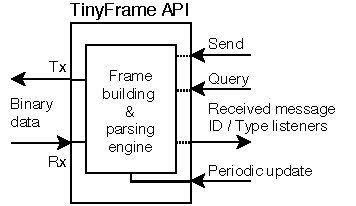
\includegraphics[scale=1]{img/tf-conceptual.pdf}
	\caption{\label{fig:tf_conceptual}TinyFrame API}
\end{wrapfigure}

GEX uses the \textit{TinyFrame}~\cite{tinyframerepo} framing library, developed, likewise, by the author, but kept as a separate project for easier re-use in different applications. The library implements frame building and parsing, including checksum calculation, and provides high-level \gls{API}.

Both peers, GEX and the client library running on the host \gls{PC}, are at an equal level: either side can independently send a message at any time. The communication is organized in transactions; a transaction consists of one or more messages going in either direction. A message can be stand-alone, or chained to another, typically a request, using the frame ID field; this is the major advantage over text-based protocols, like AT commands, where all messages are independent and their relation to each other is not always clear.

\section{Binary Payload Structure Notation}

Binary payloads are described in several places of this text. We use a shortened notation derived from the C language to represent field data types:

\begin{pldlist}
	\cfield{bool} -- 8-bit field allowing values 0 (false) and 1 (true)
	\cfield{u8}, \cfieldx{u16}, \cfieldx{u32}  -- unsigned 8-, 16-, or 32-bit integer
	\cfield{i8}, \cfieldx{i16}, \cfieldx{i32}  -- signed (two's complement) 8-, 16-, or 32-bit integer
	\cfield{char} -- an 8-bit ASCII character
	\cfield{float} -- single-precision (32-bit) IEEE~754~\cite{floatpaper} floating point number
	\cfield{double} -- double-precision (64-bit) IEEE~754~\cite{floatpaper} floating point number
	\cfield{u8[]} -- array of variable length
	\cfield{u8[n]} -- array of length n
	\cfield{cstring} -- zero-terminated character string (like \cfieldx{char[]}, ending with a 0x00 byte)
\end{pldlist}


\section{Frame Structure}

Message frames have the following structure (all little-endian):

\begin{boxedpayload}[``TinyFrame'' frame structure, as used in GEX]
	\cfield{0x01} start-of-frame marker
	\cfield{u16} frame ID
	\cfield{u16} payload length
	\cfield{u8} frame type
	\cfield{u8} header checksum
	\cfield{u8[]} payload
	\cfield{u8} payload checksum (omitted for empty payloads)
\end{boxedpayload}

\iffalse
\begin{table}[h]
	\centering
	%\hspace{-1.5em}
	\begin{tabular}{rccccccc}
		\toprule
		\multicolumn{1}{c|}{} &
		\multicolumn{5}{c}{Header}&
		\multicolumn{2}{|c}{Body} \\
		\midrule
		%
		\textit{Field} &
			\textbf{SOF} &
			\textbf{Frame ID} &
			\makecell{ \Gape{\textbf{Payload}} \\ \Gape{\textbf{Length}} } &
			\makecell{ \textbf{Frame} \\ \textbf{type} } &
			\makecell{ \textbf{Header} \\ \textbf{checksum} } &
			\textbf{Payload} &
			\makecell{ \textbf{Payload} \\ \textbf{checksum} } \\
		%
		\midrule
		\textit{Bytes} &
			 1  &
			 2  &
			 2  &
			 1  &
			 1  &
			 ... &
			 1 \\
		%
		\bottomrule
	\end{tabular}
\end{table}
\fi

\textit{Frame ID}, which could be better described as \textit{Transaction ID}, uniquely identifies each transaction. The most significant bit is set to a different value in each peer to avoid ID conflicts, and the rest of the ID field is incremented with each initiated transaction.

\section{Message Listeners} \label{sec:tf_listeners}

After sending a message that should receive a response, the peer registers an \textit{ID listener} with the ID of the sent message. A response reuses the original frame ID and when it is received, this listener is called to process it. ID listeners can also be used to receive multi-part messages re-using the original ID.

\textit{Frame type} describes the payload and does not have any prescribed format in TinyFrame; its values are defined by the application. A \textit{type listener} may be registered to handle all incoming messages with a given frame type. It works in a similar way to an ID listener, but has a lower priority.

Each message can be handled by only one listener, unless the listener explicitly requests it to be passed on. Messages not handled by any listener are given to a default listener, which can, e.g., write an error to a debug log.

\section{Designated Frame Types}

\Cref{fig:tf_types} lists the frame types defined by GEX. It is divided into four logical sections: General, Bulk Read/Write, Unit Access, and Settings. The payloads belonging to those frame types will be outlined in the following sections.

\begin{table}[h]
	\centering
	\begin{tabular}{clll}
		\toprule
		\textbf{Frame type} & \textbf{Function} & \textbf{Note} \\
		\midrule
		0x00 & Success & \textit{Payload depends on context} \\
		0x01 & Ping & \textit{GEX responds with Success and its version string} \\
		0x02 & Error & \textit{Payload contains the error message} \\
		\midrule
		0x03 & Bulk Read Offer & \textit{An offer of data to read using }0x04 \\
		0x04 & Bulk Read Poll & \textit{Requesting to read a block of data} \\
		0x05 & Bulk Write Offer & \textit{An offer to receive a bulk write transaction} \\
		0x06 & Bulk Data & \textit{Used for both reading and writing} \\
		0x07 & Bulk End & \textit{Marks the last ``Bulk Data'' frame} \\
		0x08 & Bulk Abort & \textit{} \\
		\midrule
		0x10 & Unit Request & \textit{Request to a unit} \\
		0x11 & Unit Report & \textit{Spontaneous event generated by a unit} \\
		\midrule
		0x20 & List Units & \textit{Read a list of all instantiated units} \\
		0x21 & INI Read & \textit{Request a bulk read transaction of an INI file} \\
		0x22 & INI Write & \textit{Request a bulk write transaction of an INI file} \\
		0x23 & Persist Config & \textit{Write updated configuration to flash} \\
		\bottomrule
	\end{tabular}
\caption{\label{fig:tf_types}Frame types used by GEX}
\end{table}


\section{Bulk Read and Write Transactions} \label{sec:tf_bulk_rw}

The bulk read and write transactions are generic, multi-message exchanges which are used to transfer the INI configuration files. They could additionally be used by some future unit requiring to transfer a large amount of data (e.g., to read image data from a camera).

The reason for splitting a long file into multiple messages, rather than sending it all in one, lies in the hardware limitations of the platform, specifically its small amount of \gls{RAM} (the STM32F072 has only 16\,kB). A message cannot be processed until its payload checksum is received and verified; however, the configuration file can have several kilobytes, owning to the numerous explanatory comments, which would require a prohibitively large data buffer. The chunked transaction could, additionally, be extended to support message re-transmission on timeout without sending the entire file again.

A read or write transaction can be aborted by a frame \CmdBulkAbort at any time, though aborting a write transaction may leave the configuration in a corrupted state. As hinted in the introduction of this chapter, a transaction is defined by sharing a common frame ID. Thus, all frames in a bulk transaction must have the same ID, otherwise the ID listeners would not be called for the subsequent messages.

\Cref{fig:bulk_rw} shows a diagram of the bulk read and write data flow.

\begin{figure}
	\centering
	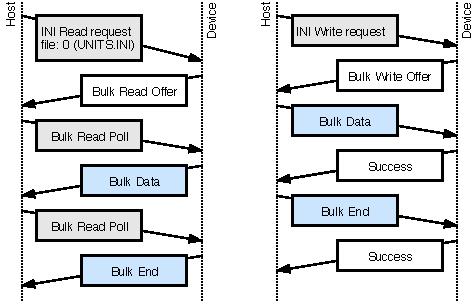
\includegraphics[scale=1.5]{img/bulk-read-write.pdf}
	\caption{\label{fig:bulk_rw}A diagram of the bulk read and write transaction.}
\end{figure}

\subsection{Bulk Read}

To read an INI file, we first send a frame \CmdINIRead, specifying the target file in the payload:

\begin{boxedpayload}[Frame \CmdINIRead payload structure]
	\cfield{u8} which file to write
		\begin{pldlist}
			\item 0 \dots UNITS.INI
			\item 1 \dots SYSTEM.INI
		\end{pldlist}
\end{boxedpayload}

What follows is a standard bulk read transaction with the requested file.
GEX offers the file for reading with a frame \CmdBulkReadOffer:

\begin{boxedpayload}[Frame \CmdBulkReadOffer payload structure]
	\cfield{u32} full size of the file in bytes
	\cfield{u32} largest chunk that can be read at once
\end{boxedpayload}

Now we can proceed to read the file using \CmdBulkReadPoll, which is always responded to with \CmdBulkData, or \CmdBulkEnd if this was the last frame. Data frames have only the useful data as their payload. The \CmdBulkReadPoll payload specifies how many bytes we want to read:

\begin{boxedpayload}[Frame \CmdBulkReadPoll payload structure]
	\cfield{u32} how many bytes to read (at most)
\end{boxedpayload}

\begin{boxedpayload}[Frame \CmdBulkData or \CmdBulkEnd payload in a ``read'' transaction]
\cfield{char[]} a chunk of the read file
\end{boxedpayload}

\subsection{Bulk Write}

To overwrite an INI file, we first send a frame \CmdINIWrite with the file size as its payload. The name of the file is irrelevant, as it is detected automatically by inspecting the content.

\begin{boxedpayload}[Frame \CmdINIWrite payload structure]
	\cfield{u32} size of the written file, in bytes
\end{boxedpayload}

\noindent
The write request is confirmed by a frame \CmdBulkWriteOffer sent back:

\begin{boxedpayload}[Frame \CmdBulkWriteOffer payload structure]
	\cfield{u32} total bytes to write (here copied from the request frame)
	\cfield{u32} how many bytes may be written per message
\end{boxedpayload}

We can now send the file as a series of frames of type \CmdBulkData, or \CmdBulkEnd in the last frame, with chunks of the data as their payloads. Each frame is confirmed by \CmdSuccess.

\begin{boxedpayload}[Frame \CmdBulkData or \CmdBulkEnd payload in a ``write'' transaction]
	\cfield{char[]} a chunk of the written file
\end{boxedpayload}

\subsection{Persisting the Changed Configuration to Flash}

The written INI file is immediately parsed and the settings are applied. However, those changes are not persistent: they exist only in RAM and will be lost when the module restarts. To save the current state to Flash, issue a frame \CmdPersistConfig. This has the same effect as pressing the LOCK button (or replacing the LOCK jumper) when the INI files are edited using the virtual mass storage.

It should be noted that after flashing a firmware, the Flash control registers may remain in an unexpected state and the module must first be manually restarted before attempting to persist settings. Otherwise an assertion will fail and the module is restarted by a watchdog, losing the temporary changes.

% TODO there must be a workaround, and then this paragraph can be removed.


\section{Reading a List of Units}

The frame \CmdListUnits requests a list of all available units in the GEX module. The list includes all units' callsigns, names and types. The response payload has the following format:

\begin{boxedpayload}[Frame \CmdListUnits response structure]
	\cfield{u8} the number of available units
	\item For each unit:
		\begin{pldlist}
			\cfield{u8} unit callsign
			\cfield{cstring} unit name
			\cfield{cstring} unit type
		\end{pldlist}
\end{boxedpayload}


\section{Unit Requests and Reports} \label{sec:unit_requests_reports}

Frame types \CmdUnitRequest and \CmdUnitReport are dedicated to messages sent to and by unit instances. Each has a fixed header (\textit{inside the payload}) followed by unit-specific data.

\subsection{Unit Requests}\label{sec:unit_requests_format}

Unit requests deliver a message from the host to a unit instance. Unit drivers implements different commands, each with its own payload structure. The frame \CmdUnitRequest has the following structure:

\begin{boxedpayload}[Frame \CmdUnitRequest payload structure]
	\cfield{u8} unit callsign
	\cfield{u8} command number, handled by the unit driver
	\cfield{u8[]} command payload, handled by the unit driver; its size and content depend on the unit driver and the particular command number, as defined in \cref{sec:units_overview}
\end{boxedpayload}

The most significant bit of the command byte (0x80) has a special meaning: when set, the message delivering routine responds with 0x00 (Success) after the command completes, unless an error occurred. That is used to get a confirmation that the message was delivered and the module operates correctly (as opposed to, e.g., a lock-up resulting in a watchdog reset). Requests which normally generate a response (e.g., reading a value from the unit) should not be sent with this flag, as that would produce two responses at once.

\subsection{Unit Reports}\label{sec:unit_reports_format}

Several unit types can produce asynchronous events, such as reporting a pin change, or a triggering condition. The event is timestamped and sent with a frame type \CmdUnitReport:

\begin{boxedpayload}[Frame \CmdUnitReport payload structure]
	\cfield{u8} unit callsign
	\cfield{u8} report type, defined by the unit driver
	\cfield{u64} event time (microseconds since power-on)
	\cfield{u8[]} report payload; similar to requests, the payload structure depends on the unit driver and the particular report type, as defined in \cref{sec:units_overview}
\end{boxedpayload}

















